\documentclass[a4paper,12pt]{article}
\usepackage[latin1]{inputenc}
\usepackage[T1]{fontenc}
\usepackage{textcomp}
\usepackage{eurosym}

\usepackage{tabularx}
\usepackage{multirow}

\usepackage{amsmath}
\usepackage{amssymb}
\usepackage{amscd} 
\usepackage[all,cmtip]{xy}

\usepackage{graphicx} 

\setlength\overfullrule{5pt}

\newcommand{\pois}[1]{}

\title{ Weekly Exercise 6}
\author{Shubo Yan }
\date{4.10.2017}


\begin{document}
\maketitle
\newpage
\section*{Exercise 1}

\subsection*{Solving an equation of 3rd degree} 

By \emph{Vieta\!'s formula} it is possible to solve an equation of 3rd degree. 

Let the original equation be 
\begin{align}
ax^{3}+bx^{2}+cx=0 \text{,\hspace{2cm}where }a\ne 0
\end{align}
Doing $x\displaystyle\leftarrow t-\frac{b}{3a}$ (\emph{T\!schirnhaus transformation}) we get for \emph{the equation to be solved}:
\begin{equation}
t^{3}+pt+q=0 
\end{equation}
By using \emph{Vieta\!'s formula}
\begin{align}
t=w-\frac{p}{3w}&\text{,\hspace{2cm}where }w\ne 0\text{,}
\end{align}
we get the equation
\begin{align}
w^{3}+q-\frac{p^{3}}{27w^{3}}=0\text{,}
\end{align}
By multiplying both sides by $w^{3}$ we get \emph{an equation of 6th degree} but actually it is 2nd degree of $w^{3}$:
\begin{equation}
w^{6}+qw^{3}-\frac{p^{3}}{27}=0\text{,}
\end{equation}
Let us solve this for $w^{3}$. Let $w_1$, $w_2$, and $w_3$ $w^{3}$ be the \emph{the cubic roots}.
\begin{quote}
All real numbers, except $0$, have exactly one \emph{real} cubic root, and two complex conjugates, and all non-zero complex numbers have three distinct complex cubic roots. \\
For example:

\begin{subequations}
	\begin{align}
	\sqrt[3]{0}&=0 \\
	\sqrt[3]{8}&=\begin{cases}
	                   2\\
                       -1-i\sqrt[2]{3}\\
                       -1+i\sqrt[2]{3}
	             \end{cases}\\
	\sqrt[3]{-27i}&=\begin{cases} 
	                 3i \\
	                  \frac{3\sqrt{3}}{2}-\frac{3}{2}i\\
	                  -\frac{3\sqrt{3}}{2}-\frac{3}{2}i
	                 \end{cases}           
    \end{align}
\end{subequations}
\end{quote}
Now the roots of equation (2) are
\begin{subequations}
	\begin{align}
	t_1&=w-\frac{p_1}{3w_1}\text{,}\\
	t_2&=w-\frac{p_2}{3w_2}\text{, and}\\
	t_3&=w-\frac{p_3}{3w_3}\text{ .}
	\end{align}
\end{subequations}

\section*{Exercise 2}
\bigskip

Let
\begin{equation}
A=
\begin{pmatrix}
a_{11}&a_{12}&a_{13}\\
a_{21}&a_{22}&a_{23}\\
a_{31}&a_{32}&a_{33}
\end{pmatrix}
=  
\begin{pmatrix}
1&2&3\\
4&5&6\\
7&8&9
\end{pmatrix}
\end{equation}
The adjungated matrix is computed as follows:
\begin{equation}
\mathsf{adj}(A)=
\begin{pmatrix}
	+\begin{vmatrix}a_{22}&a_{23}\\a_{32}&a_{33}\end{vmatrix}&
	-\begin{vmatrix}a_{21}&a_{23}\\a_{31}&a_{33}\end{vmatrix}&
	+\begin{vmatrix}a_{21}&a_{21}\\a_{32}&a_{33}\end{vmatrix}\\[2em]
	-\begin{vmatrix}a_{12}&a_{13}\\a_{32}&a_{33}\end{vmatrix}&
	+\begin{vmatrix}a_{11}&a_{13}\\a_{31}&a_{33}\end{vmatrix}&
	-\begin{vmatrix}a_{11}&a_{12}\\a_{32}&a_{33}\end{vmatrix}\\[2em]
	+\begin{vmatrix}a_{12}&a_{13}\\a_{22}&a_{23}\end{vmatrix}&
	-\begin{vmatrix}a_{11}&a_{12}\\a_{31}&a_{32}\end{vmatrix}&
	+\begin{vmatrix}a_{11}&a_{12}\\a_{21}&a_{22}\end{vmatrix}\\
\end{pmatrix}
\end{equation}

Thus
\begin{equation}
\mathsf{adj}
\begin{pmatrix}
	-3&2&-5\\
	-1&0&-2\\
	 3&-4&1
\end{pmatrix}
=
\begin{pmatrix}
-8&18&-4\\
-5&12&-1\\
4&-6&2
\end{pmatrix}
\end{equation}

\section*{Exercise 3}

\[
\xymatrix{
A\ar@{-}[rr]\ar@{-}[dr]\ar@{-}[dd]
&&B\ar@{-}[dd]|\hole\ar@{-}[dr]\\
&E\ar@{-}[rr]\ar@{-}[dd]
&&F\ar@{-}[dd]\\C\ar@{-}[rr]|\hole
\ar@{-}[dr]
&&D\ar@{-}[dr]\\
&G\ar@{-}[rr]\ar@{-}[ul]
&&H
}
\]
\section*{Exercise 4}
\begin{figure}[b!]
\centering
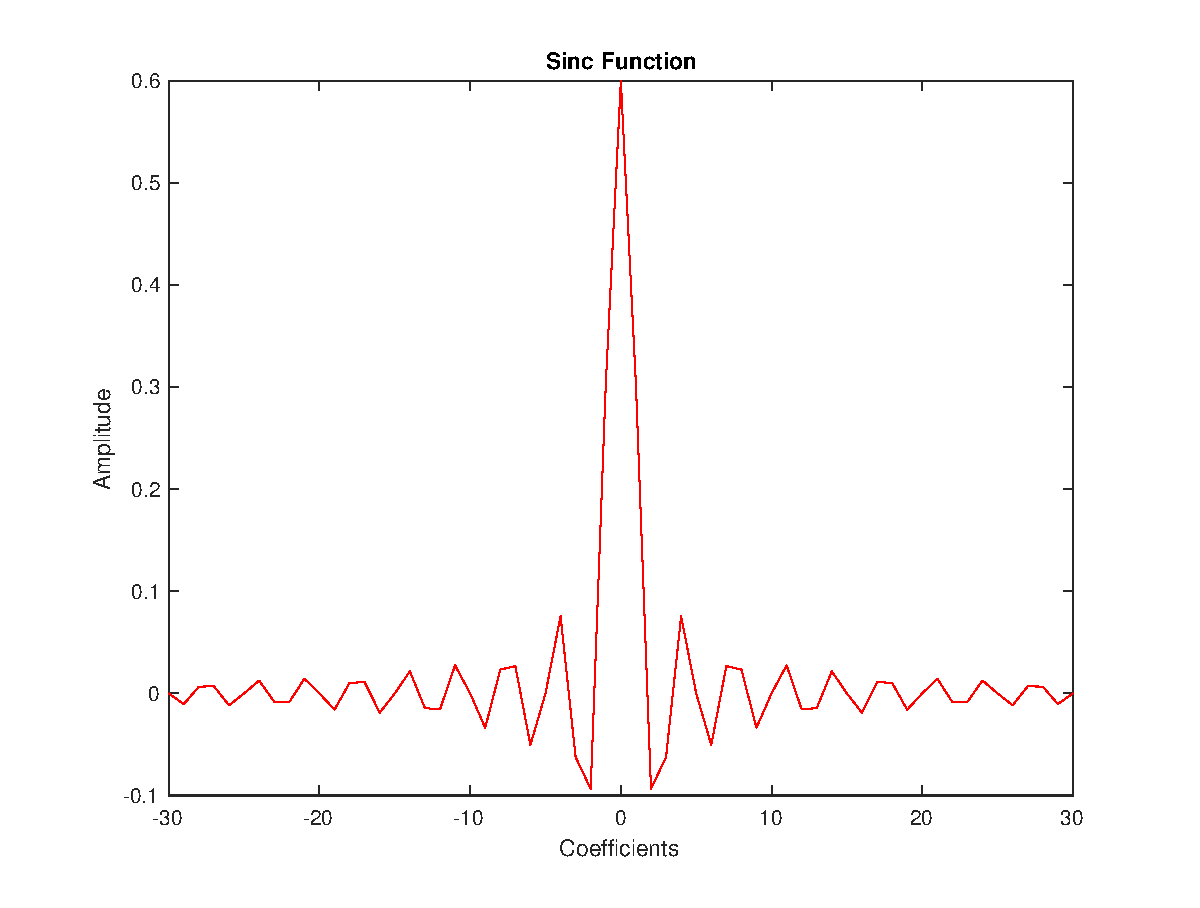
\includegraphics[width=\textwidth]{sinc.eps}
%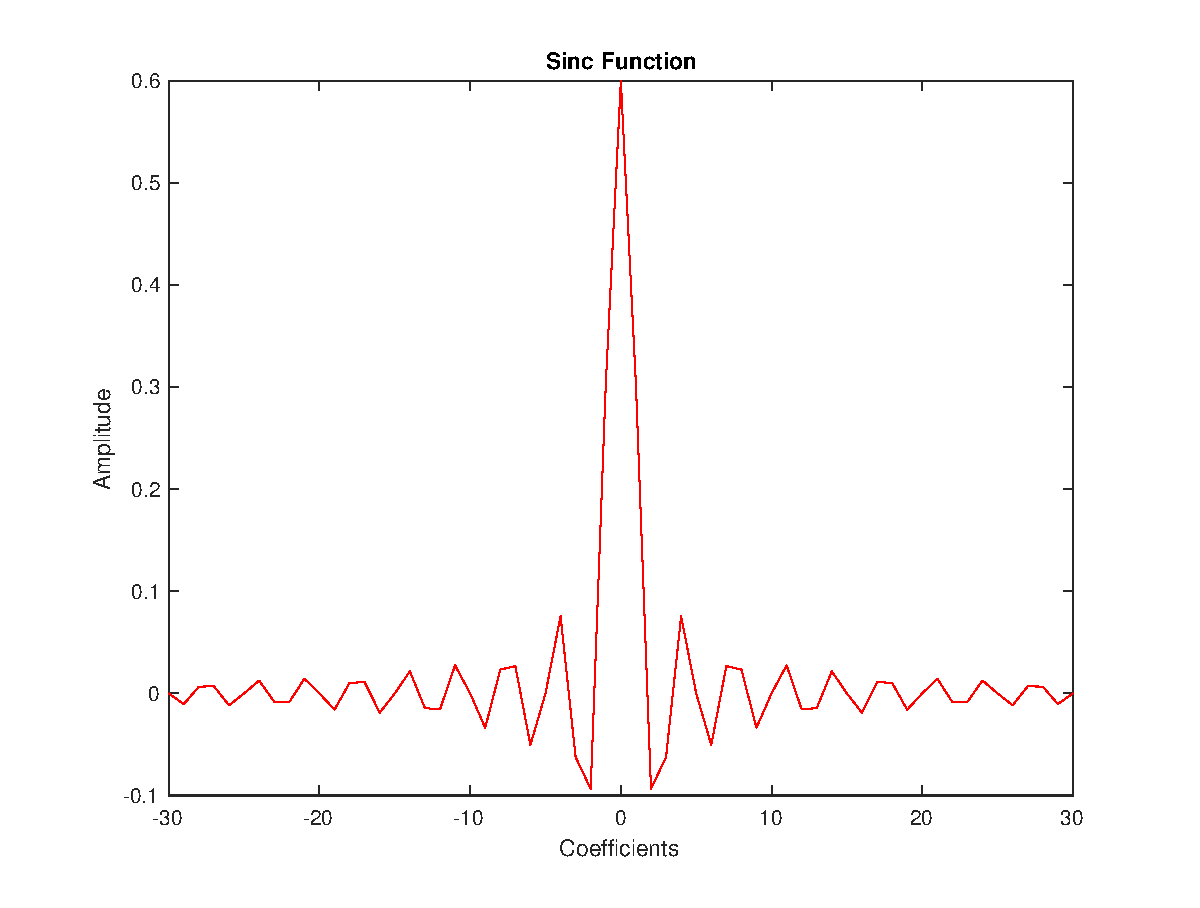
\includegraphics[width=5cm,angle=30]{sinc.eps}
\caption{\textquotedblleft interesting\textquotedblright curve}
\end{figure}
\pagebreak

\section*{Exercise 5}
\begin{figure}[b!]
\setlength{\unitlength}{1mm}
\centering
\begin{picture}(120,120)(-10,-10)
\put(-10,-10){\framebox(120,120){}}
\multiput(0,0)(1,0){101}{\line(0,1){100}}
\multiput(0,0)(0,1){101}{\line(1,0){100}}
{\linethickness{1pt}
\multiput(0,0)(5,0){21}{\line(0,1){100}}
\multiput(0,0)(0,5){21}{\line(1,0){100}}
}
{\linethickness{2pt}
	\multiput(0,0)(10,0){11}{\line(0,1){100}}
	\multiput(0,0)(0,10){11}{\line(1,0){100}}
}
{\linethickness{4pt}
	\put(0,0){\framebox(100,100){}}
}
\put(0,-5){\makebox(0,0){0}}
\put(10,-5){\makebox(0,0){1}}
\put(20,-5){\makebox(0,0){2}}
\put(30,-5){\makebox(0,0){3}}
\put(40,-5){\makebox(0,0){4}}
\put(50,-5){\makebox(0,0){5}}
\put(60,-5){\makebox(0,0){6}}
\put(70,-5){\makebox(0,0){7}}
\put(80,-5){\makebox(0,0){8}}
\put(90,-5){\makebox(0,0){9}}
\put(100,-5){\makebox(0,0){10}}

\put(-4,0){\makebox(0,0)[r]{0}}
\put(-4,10){\makebox(0,0)[r]{1}}
\put(-4,20){\makebox(0,0)[r]{2}}
\put(-4,30){\makebox(0,0)[r]{3}}
\put(-4,40){\makebox(0,0)[r]{4}}
\put(-4,50){\makebox(0,0)[r]{5}}
\put(-4,60){\makebox(0,0)[r]{6}}
\put(-4,70){\makebox(0,0)[r]{7}}
\put(-4,80){\makebox(0,0)[r]{8}}
\put(-4,90){\makebox(0,0)[r]{9}}
\put(-4,100){\makebox(0,0)[r]{10}}
\end{picture}	
\caption{mm grid}
\end{figure}
\end{document}